\Opensolutionfile{solution_file}[solutions/sols_010]
% в квадратных скобках фактическое имя файла

\chapter{МНК без матриц и вероятностей}

\begin{problem} %1.1
Пусть $a = (a_1,\dots,a_n)$ и $b = (b_1,\dots,b_n)$ — два произвольных вектора. Определите, какие равенства справедливы:
\begin{enumerate}
\item $\sum_{i=1}^n {(a_i-\bar a)} = 0$;
\item $\sum_{i=1}^n {(a_i-\bar a)^2} = \sum_{i=1}^n {(a_i-\bar a)a_i}$;
\item $\sum_{i=1}^n {(a_i-\bar a)(b_i-\bar b)} = \sum_{i=1}^n {(a_i-\bar a)b_i}$;
\item $\sum_{i=1}^n {(a_i-\bar a)(b_i-\bar b)} = \sum_{i=1}^n {a_i b_i}$;
\item $\sum_{i=1}^n a_i = n\bar a$;
\item $\sum_{i=1}^n (a_i - \bar a)^2 = \sum_{i=1}^n a_i^2 - n \bar a^2$;
\item $\sum_{i=1}^n a_i^2 = \left( \sum_{i=1}^n a_i \right)^2$;
\item $\sum_{i=1}^n a_i^2 = (n\bar a)^2$;
\item $\sum_{i=1}^n \bar a = n \bar a$;
\item $\sum_{i=1}^n a_i \bar a = n \bar a^2$;
\item $\sum_{i=1}^n {(a_i-\bar a)b_i} = 0$.
\end{enumerate}


\begin{sol}
\begin{enumerate}
\item Верно: \[\sum_{i=1}^{n}(a_i-\bar{a}) = \sum_{i=1}^{n}a_i - n\cdot\bar{a} = \sum_{i=1}^{n}a_i - \sum_{i=1}^{n}a_i = 0\]
\item Верно: \[\sum_{i=1}^{n}(a_i-\bar{a})^2 = \sum_{i=1}^{n}(a_i-\bar{a})(a_i+\bar{a}) = \sum_{i=1}^{n}(a_i-\bar{a})a_i + \bar{a}\underbrace{\sum_{i=1}^{n}(a_i-\bar{a})}_{=0} = \sum_{i=1}^{n}(a_i-\bar{a})a_i \]

\item Верно: \[\sum_{i=1}^{n}(a_i-\bar{a})(b_i-\bar{b}) = \sum_{i=1}^{n}(a_i-\bar{a})b_i - \bar{b}\underbrace{\sum_{i=1}^{n}(a_i-\bar{a})}_{=0} = \sum_{i=1}^{n}(a_i-\bar{a})b_i \]
\item А вот это неверно! (следует из предыдущего пункта)
\item Верно
\item Верно
\item Неверно
\item Неверно
\item Верно
\item Верно: \[\sum_{i=1}^{n}a_i\bar{a} = \frac{n}{n}\bar{a}\sum_{i=1}^{n}a_i = n \bar{a} \frac{\sum_{i=1}^{n}a_i}{n} = n\bar{a}^2 \]
\item Неверно (см. пунк 3)
\end{enumerate}
\end{sol}
\end{problem}





\begin{problem} %1.2
При помощи метода наименьших квадратов найдите оценку неизвестного параметра $\theta$ в следующих моделях:

\begin{enumerate}
\item $y_i = \theta + \theta x_i + \varepsilon_i$;
\item $y_i = \theta - \theta x_i + \e_i$;
\item $\ln y_i = \theta + \ln x_i + \e_i$;
\item $y_i = \theta + x_i + \e_i$;
\item $y_i = 1 + \theta x_i + \e_i$;
\item $y_i = \theta / x_i + \e_i$;
\item $y_i = \theta x_i + (1-\theta)z_i+\e_i$.
\end{enumerate}


\begin{sol}
\begin{enumerate}
\item \(\htheta = \sum y_i (1 + x_i) / \sum (1 + x_i)^2\)

Стандартная процедура МНК:
\[RSS = \sum \e_i^2 = \sum \left(y_i - \theta - \theta x_i\right)^2 \rightarrow \min \limits_\theta\]
\[\frac{\partial RSS}{\partial \theta} = 2 \sum \left(y_i - \theta - \theta x_i\right)(-1 - x_i) \]
\[\sum \left(y_i - \htheta - \htheta x_i\right)(-1 - x_i) = 0\]
\[\sum y_i (-1 - x_i) + \htheta \sum (-1 - x_i)^2 = 0 \]
\[\htheta = \frac{\sum y_i (1 + x_i)}{\sum (1 + x_i)^2} \]

\item \(\htheta = \sum \left(y_i (1 - x_i)\right) / \sum (1 - x_i)^2\)

\item \(\htheta = \left( \sum \text{ln} (y_i / x_i) \right) / n \)

\item \(\htheta = \left( \sum (y_i - x_i) \right) / n \)

\item \(\htheta = \sum \left((y_i - 1) x_i\right) / \sum x_i^2\)

\item \(\htheta = \sum (y_i / x_i^2) / \sum (1 /x^3)\)

\item \(\htheta = \sum \left((y_i - z_i)(x_i - z_i) \right) / \sum \left(x_i - z_i\right)^2 \)

\end{enumerate}
\end{sol}
\end{problem}


\begin{problem} %1.3
Покажите, что для моделей $y_i= \alpha + \beta x_i + \e_i$, $z_i = \gamma + \delta x_i + \upsilon_i$ и $y_i + z_i = \mu + \lambda x_i + \xi_i$ МНК-оценки связаны соотношениями $\hat{\mu}=\hat{\alpha}+\hat{\gamma}$ и $\hat{\lambda}=\hb + \hat{\delta}$.


\begin{sol}
Заметим, что $y_i + z_i = \underbrace{(\alpha + \gamma)}_{\mu} + \underbrace{(\beta+\delta)}_{\lambda}x_i + u_i$.

Если оценить данную модель при помощи МНК, получим как раз то, что нужно доказать.
\end{sol}
\end{problem}


\begin{problem} %1.4
Найдите МНК-оценки параметров $\alpha$ и $\beta$ в модели $y_i = \alpha + \beta y_i + \e_i$.


\begin{sol}
\(\hat{\alpha} = 0, \ \hb = 1 \)
\end{sol}
\end{problem}


\begin{problem} %1.5
Рассмотрите модели $y_i = \alpha + \beta (y_i + z_i) + \e_i$, $z_i = \gamma + \delta(y_i+z_i) + \e_i$.
\begin{enumerate}
\item Как связаны между собой $\hat{\alpha}$ и $\hat{\gamma}$?
\item Как связаны между собой $\hb$ и $\hat{\delta}$?
\end{enumerate}


\begin{sol} % 1.5.
Рассмотрим регрессию суммы $(y_i + z_i)$ на саму себя. Естественно, в ней
\[
\widehat{y_i + z_i} = 0 + 1 \cdot (y_i + z_i).
\]

Отсюда получаем, что $\hat{\alpha} + \hat{\gamma} = 0$ и $\hb + \hat{\delta} = 1$.
\end{sol}
\end{problem}




\begin{problem} %1.6
Как связаны МНК-оценки параметров $\alpha, \beta$ и $\gamma, \delta$ в моделях $y_i = \alpha + \beta x_i + \e_i$ и $z_i = \gamma + \delta x_i + \upsilon_i$, если $z_i = 2 y_i$?


\begin{sol}

Исходя из условия, нужно оценить методом МНК коэффициенты двух следующих моделей:
\[y_i = \alpha + \beta x_i + \e_i \]
\[y_i = \frac{\gamma}{2} + \frac{\delta}{2} x_i + \frac{1}{2} v_i \]

Заметим, что на минимизацию суммы квадратов остатков коэффициент \(1/2\) не влияет, следовательно:
\[\hat{\gamma} = 2\hat{\alpha}, \ \hat{\delta} = 2 \hb  \]

\end{sol}
\end{problem}


\begin{problem} %1.6
Для модели $y_i = \beta_1 x_i + \beta_2 z_i + \e_i$ решите условную задачу о наименьших квадратах:
\[
Q(\beta_1, \beta_2) := \sum_{i=1}^n (y_i - \beta_1 x_i - \beta_2 z_i)^2 \rightarrow \underset{\beta_1 + \beta_2 = 1}{\min}.
\]


\begin{sol}
Выпишем задачу:
\[
\begin{cases}
RSS = \sum\limits_{i=1}^{n}(y_i - \beta_1x_i - \beta_2z_i)^2 \rightarrow \min\limits_{\beta_1, \beta_2}\\
\beta_1 + \beta_2 = 1
\end{cases}
\]

Можем превратить ее в задачу минимизации функции одного аргумента:
\[
RSS =  \sum\limits_{i=1}^{n}(y_i - x_i - \beta_2(z_i-x_i))^2 \rightarrow \min_{\beta_2}
\]

Выпишем условия первого порядка:
\[
\frac{\partial RSS}{\partial \beta_2} = \sum\limits_{i=1}^{n}2(y_i-x_i-\hb_2(z_i-x_i))(x_i-z_i)=0
\]

Отсюда:
\[
\sum\limits_{i=1}^{n}(y_i-x_i)(x_i-z_i) + \hb_2\sum\limits_{i=1}^{n}(z_i-x_i)^2 = 0 \Rightarrow \hb_2 = \frac{\sum\limits_{i=1}^n (y_i-x_i)(z_i-x_i)}{\sum\limits_{i=1}^n (z_i-x_i)^2}
\]

А оценка $\beta_1$ найдется из соотношения $\hb_1+\hb_2 = 1$.

\end{sol}
\end{problem}




\begin{problem} %1.8
Даны $n$ пар чисел: $(x_1, y_1)$, \ldots, $(x_n,y_n)$. Мы прогнозируем $y_i$ по формуле $\hy_i=\hb x_i$. Найдите $\hb$ методом наименьших квадратов.


\begin{sol}
$\hb=\sum x_i y_i/\sum x_i^2$
\end{sol}
\end{problem}


\begin{problem} %1.9
Даны $n$ чисел: $y_1$, \ldots, $y_n$. Мы прогнозируем $y_i$ по формуле $\hy_i=\hb$. Найдите $\hb$ методом наименьших квадратов.

\begin{sol}
Нужно решить задачу:
\[
RSS = \sum\limits_{i=1}^n(y_i-\beta)^2 \rightarrow \min\limits_{\beta}
\]

Условия первого порядка:
\[
\frac{\partial RSS}{\partial \beta} = \sum\limits_{i=1}^{n}2(y_i-\hb) = 0 \Rightarrow \sum\limits_{i=1}^n y_i-n\hb = 0
\]

Поэтому
\[
\hb = \frac{\sum_{i=1}^ny_i}{n} = \bar{y}
\]
\end{sol}
\end{problem}


\begin{problem} % 1.10
Даны $n$ пар чисел: $(x_1, y_1)$, \ldots, $(x_n,y_n)$. Мы прогнозируем $y_i$ по формуле $\hy_i=\hb_1+\hb_2 x_i$. Найдите $\hb_1$ и $\hb_2$ методом наименьших квадратов.

\begin{sol}
$\hb_2=\sum (x_i-\bar{x})(y_i-\bar{y})/\sum(x_i-\bar{x})^2$, $\hb_1=\bar{y}-\hb_2\bar{x}$
\end{sol}
\end{problem}


\begin{problem}%1.11
Даны $n$ пар чисел: $(x_1, y_1)$, \ldots, $(x_n,y_n)$. Мы прогнозируем $y_i$ по формуле $\hy_i=1+\hb x_i$. Найдите $\hb$ методом наименьших квадратов.

\begin{sol}
Имеем следующую задачу:
\[
RSS = \sum\limits_i(y_i-1-\beta x_i)^2 \rightarrow \min\limits_{\beta}
\]

Откуда сразу все находим:
\[
\frac{\partial RSS}{\partial \beta} = \sum\limits_i2(y_i-1-\hb x_i)(-x_i) = 0 \Rightarrow \sum\limits_i (y_i-1-\hb x_i)x_i=0 \Rightarrow
\]
\[
\sum\limits_i x_iy_i-\sum\limits_ix_i - \hb\sum\limits_ix_i^2 = 0 \Rightarrow \hb = \frac{\sum_ix_i(y_i-1)}{\sum_ix_i^2}
\]
\end{sol}
\end{problem}


\begin{problem} %1.12
Перед нами два золотых слитка и весы, производящие взвешивания с ошибками. Взвесив первый слиток, мы получили результат $300$ грамм, взвесив второй слиток — $200$ грамм, взвесив оба слитка — $400$ грамм. Оцените вес каждого слитка методом наименьших квадратов.

\begin{sol}
Обозначив вес первого слитка за \(\beta_1\), вес второго слитка за \(\beta_2\), а показания весов за \(y_i\), получим, что
\[y_1 = \beta_1 + \e_1, \ y_2 = \beta_2 + \e_2, \ y_3 = \beta_1 + \beta_2 + \e_3\]

Тогда
\[(300 - \beta_1)^2 + (200 - \beta_2)^2 + (400 - \beta_1 - \beta_2)^2 \rightarrow \min \limits_{\beta_1,\  \beta_2} \]
\[\hb_1 = \frac{800}{3}, \ \hb_2 = \frac{500}{3} \]
\end{sol}
\end{problem}



\begin{problem} %1.13
Аня и Настя утверждают, что лектор опоздал на 10 минут. Таня считает, что лектор опоздал на 3 минуты. С помощью МНК оцените, на сколько минут опоздал лектор.

\begin{sol}

Ане, Насте и Тане нужно оценить модель $y_i = \beta + \e_i$. Для этого они должны решить следующую задачу:

\[RSS = 2(10-\beta)^2 + (3-\beta)^2\rightarrow \min \limits_{\beta}\]

\[\frac{\partial RSS}{\partial \beta} = -4(10-\beta)-2(3-\beta) \]

Условия первого порядка:

\[-4(10-\hb)-2(3-\hb)=0\]

\[20 - 2\hb +3 -\hb=0\]

\[3\hb = 23\]

\[\hb = \frac{23}{3}\]

\end{sol}
\end{problem}



\begin{problem} %1.14
Функция $f(x)$ непрерывна на отрезке $[0;1]$. Найдите аналог МНК-оценок для регрессии без свободного члена в непрерывном случае. Более подробно: найдите минимум по $\hb$ для функции
\[
Q(\hb)= \int_0^1 (f(x)-\hb x)^2\,dx.
\]

\begin{sol}
Условие первого порядка $\int_0^1 -2x(f(x)-\hb x) \, dx =0$, получаем
\[
\hb = \frac{\int_0^1 x f(x)\, dx} {\int_0^1 x^2 \, dx}
\]

\(\hb = \left(\int \limits_0^1 f(x) x dx\right) / \left(\int \limits_0^1 x^2 dx\right)\)
\end{sol}
\end{problem}



\begin{problem} %1.15
Есть двести наблюдений. Вовочка оценил модель $\hy=\hb_1+\hb_2 x$ по первой сотне наблюдений. Петечка оценил модель $\hy=\hat{\gamma}_1+\hat{\gamma}_2 x$ по второй сотне наблюдений. Машенька оценила модель $\hy=\hat{m}_1+\hat{m}_2 x$ по всем наблюдениям.
\begin{enumerate}
\item Возможно ли, что $\hb_2>0$, $\hat{\gamma}_2>0$, но $\hat{m}_2<0$?
\item Возможно ли, что $\hb_1>0$, $\hat{\gamma}_1>0$, но $\hat{m}_1<0$?
\item Возможно ли одновременное выполнение всех упомянутых условий?
\end{enumerate}


\begin{sol}
\begin{enumerate}
\item Проявите воображение! Все зависит от данных. Например, может быть вот так:

\begin{minted}[mathescape,
               linenos,
               numbersep=5pt,
               frame=lines,
               framesep=2mm]{r}
n <- 100;
s <- rep(c(0, 4), c(n/2, n/2));
x <- c(1 + runif(n/2), runif(n/2));
y <- 2 * x + s + rnorm(n, sd = 0.15)


plot(x, y, type = "n", frame = "FALSE")
points(x[1 : (n/2)], y[1 : (n/2)], pch = 21,
       col = "black", bg = "ForestGreen", cex = 2)
points(x[(n/2 + 1) : n], y[(n/2 + 1) : n],
       pch = 21, col = "black", bg = "SkyBlue", cex = 2)

modelV1 <- lm(y ~ x + s)
# модели по 1:100 и 101:200 в отдельности
abline(coef(modelV1)[1], coef(modelV1)[2], lwd = 3)
abline(coef(modelV1)[1] + 4 * coef(modelV1)[3],
       coef(modelV1)[2], lwd = 3)
modelV2 <- lm(y ~ x)
# общая модель
abline(modelV2, lwd = 2, col = "red")
\end{minted}

\begin{minipage}{0.6\textwidth}
\begin{center}
\begin{tikzpicture}[scale = 0.025]
% Created by tikzDevice version 0.12 on 2019-05-26 19:49:23
% !TEX encoding = UTF-8 Unicode
\begin{tikzpicture}[x=1pt,y=1pt]
\definecolor{fillColor}{RGB}{255,255,255}
\path[use as bounding box,fill=fillColor,fill opacity=0.00] (0,0) rectangle (505.89,505.89);
\begin{scope}
\path[clip] (  0.00,  0.00) rectangle (505.89,505.89);
\definecolor{drawColor}{RGB}{0,0,0}

\path[draw=drawColor,line width= 0.4pt,line join=round,line cap=round] ( 70.67, 73.44) -- (467.59, 73.44);

\path[draw=drawColor,line width= 0.4pt,line join=round,line cap=round] ( 70.67, 73.44) -- ( 70.67, 66.24);

\path[draw=drawColor,line width= 0.4pt,line join=round,line cap=round] (169.90, 73.44) -- (169.90, 66.24);

\path[draw=drawColor,line width= 0.4pt,line join=round,line cap=round] (269.13, 73.44) -- (269.13, 66.24);

\path[draw=drawColor,line width= 0.4pt,line join=round,line cap=round] (368.36, 73.44) -- (368.36, 66.24);

\path[draw=drawColor,line width= 0.4pt,line join=round,line cap=round] (467.59, 73.44) -- (467.59, 66.24);

\node[text=drawColor,anchor=base,inner sep=0pt, outer sep=0pt, scale=  1.00] at ( 70.67, 47.52) {0.0};

\node[text=drawColor,anchor=base,inner sep=0pt, outer sep=0pt, scale=  1.00] at (169.90, 47.52) {0.5};

\node[text=drawColor,anchor=base,inner sep=0pt, outer sep=0pt, scale=  1.00] at (269.13, 47.52) {1.0};

\node[text=drawColor,anchor=base,inner sep=0pt, outer sep=0pt, scale=  1.00] at (368.36, 47.52) {1.5};

\node[text=drawColor,anchor=base,inner sep=0pt, outer sep=0pt, scale=  1.00] at (467.59, 47.52) {2.0};

\path[draw=drawColor,line width= 0.4pt,line join=round,line cap=round] ( 59.04,108.92) -- ( 59.04,423.29);

\path[draw=drawColor,line width= 0.4pt,line join=round,line cap=round] ( 59.04,108.92) -- ( 51.84,108.92);

\path[draw=drawColor,line width= 0.4pt,line join=round,line cap=round] ( 59.04,187.51) -- ( 51.84,187.51);

\path[draw=drawColor,line width= 0.4pt,line join=round,line cap=round] ( 59.04,266.10) -- ( 51.84,266.10);

\path[draw=drawColor,line width= 0.4pt,line join=round,line cap=round] ( 59.04,344.70) -- ( 51.84,344.70);

\path[draw=drawColor,line width= 0.4pt,line join=round,line cap=round] ( 59.04,423.29) -- ( 51.84,423.29);

\node[text=drawColor,rotate= 90.00,anchor=base,inner sep=0pt, outer sep=0pt, scale=  1.00] at ( 41.76,108.92) {2};

\node[text=drawColor,rotate= 90.00,anchor=base,inner sep=0pt, outer sep=0pt, scale=  1.00] at ( 41.76,187.51) {3};

\node[text=drawColor,rotate= 90.00,anchor=base,inner sep=0pt, outer sep=0pt, scale=  1.00] at ( 41.76,266.10) {4};

\node[text=drawColor,rotate= 90.00,anchor=base,inner sep=0pt, outer sep=0pt, scale=  1.00] at ( 41.76,344.70) {5};

\node[text=drawColor,rotate= 90.00,anchor=base,inner sep=0pt, outer sep=0pt, scale=  1.00] at ( 41.76,423.29) {6};
\end{scope}
\begin{scope}
\path[clip] (  0.00,  0.00) rectangle (505.89,505.89);
\definecolor{drawColor}{RGB}{0,0,0}

\node[text=drawColor,anchor=base,inner sep=0pt, outer sep=0pt, scale=  1.00] at (267.35, 18.72) {x};

\node[text=drawColor,rotate= 90.00,anchor=base,inner sep=0pt, outer sep=0pt, scale=  1.00] at ( 12.96,260.14) {y};
\end{scope}
\begin{scope}
\path[clip] ( 59.04, 73.44) rectangle (475.65,446.85);
\definecolor{drawColor}{RGB}{0,0,0}
\definecolor{fillColor}{RGB}{34,139,34}

\path[draw=drawColor,line width= 0.4pt,line join=round,line cap=round,fill=fillColor] (449.54,236.44) circle (  5.40);

\path[draw=drawColor,line width= 0.4pt,line join=round,line cap=round,fill=fillColor] (447.73,247.42) circle (  5.40);

\path[draw=drawColor,line width= 0.4pt,line join=round,line cap=round,fill=fillColor] (307.31,141.17) circle (  5.40);

\path[draw=drawColor,line width= 0.4pt,line join=round,line cap=round,fill=fillColor] (374.77,187.83) circle (  5.40);

\path[draw=drawColor,line width= 0.4pt,line join=round,line cap=round,fill=fillColor] (372.75,192.22) circle (  5.40);

\path[draw=drawColor,line width= 0.4pt,line join=round,line cap=round,fill=fillColor] (300.95,130.36) circle (  5.40);

\path[draw=drawColor,line width= 0.4pt,line join=round,line cap=round,fill=fillColor] (372.25,209.67) circle (  5.40);

\path[draw=drawColor,line width= 0.4pt,line join=round,line cap=round,fill=fillColor] (313.69,152.63) circle (  5.40);

\path[draw=drawColor,line width= 0.4pt,line join=round,line cap=round,fill=fillColor] (325.00,188.13) circle (  5.40);

\path[draw=drawColor,line width= 0.4pt,line join=round,line cap=round,fill=fillColor] (369.09,178.72) circle (  5.40);

\path[draw=drawColor,line width= 0.4pt,line join=round,line cap=round,fill=fillColor] (300.68,143.51) circle (  5.40);

\path[draw=drawColor,line width= 0.4pt,line join=round,line cap=round,fill=fillColor] (451.84,278.36) circle (  5.40);

\path[draw=drawColor,line width= 0.4pt,line join=round,line cap=round,fill=fillColor] (368.17,190.91) circle (  5.40);

\path[draw=drawColor,line width= 0.4pt,line join=round,line cap=round,fill=fillColor] (391.25,192.87) circle (  5.40);

\path[draw=drawColor,line width= 0.4pt,line join=round,line cap=round,fill=fillColor] (416.77,213.99) circle (  5.40);

\path[draw=drawColor,line width= 0.4pt,line join=round,line cap=round,fill=fillColor] (391.55,205.46) circle (  5.40);

\path[draw=drawColor,line width= 0.4pt,line join=round,line cap=round,fill=fillColor] (453.73,270.56) circle (  5.40);

\path[draw=drawColor,line width= 0.4pt,line join=round,line cap=round,fill=fillColor] (285.08,130.40) circle (  5.40);

\path[draw=drawColor,line width= 0.4pt,line join=round,line cap=round,fill=fillColor] (274.71, 88.13) circle (  5.40);

\path[draw=drawColor,line width= 0.4pt,line join=round,line cap=round,fill=fillColor] (376.60,185.78) circle (  5.40);

\path[draw=drawColor,line width= 0.4pt,line join=round,line cap=round,fill=fillColor] (317.00,146.73) circle (  5.40);

\path[draw=drawColor,line width= 0.4pt,line join=round,line cap=round,fill=fillColor] (397.11,193.09) circle (  5.40);

\path[draw=drawColor,line width= 0.4pt,line join=round,line cap=round,fill=fillColor] (344.10,176.48) circle (  5.40);

\path[draw=drawColor,line width= 0.4pt,line join=round,line cap=round,fill=fillColor] (278.43, 87.27) circle (  5.40);

\path[draw=drawColor,line width= 0.4pt,line join=round,line cap=round,fill=fillColor] (278.68,118.18) circle (  5.40);

\path[draw=drawColor,line width= 0.4pt,line join=round,line cap=round,fill=fillColor] (460.22,255.65) circle (  5.40);

\path[draw=drawColor,line width= 0.4pt,line join=round,line cap=round,fill=fillColor] (314.08,138.73) circle (  5.40);

\path[draw=drawColor,line width= 0.4pt,line join=round,line cap=round,fill=fillColor] (271.39,107.37) circle (  5.40);

\path[draw=drawColor,line width= 0.4pt,line join=round,line cap=round,fill=fillColor] (312.49,146.97) circle (  5.40);

\path[draw=drawColor,line width= 0.4pt,line join=round,line cap=round,fill=fillColor] (280.23,122.39) circle (  5.40);

\path[draw=drawColor,line width= 0.4pt,line join=round,line cap=round,fill=fillColor] (315.76,143.20) circle (  5.40);

\path[draw=drawColor,line width= 0.4pt,line join=round,line cap=round,fill=fillColor] (349.05,149.53) circle (  5.40);

\path[draw=drawColor,line width= 0.4pt,line join=round,line cap=round,fill=fillColor] (271.97, 94.20) circle (  5.40);

\path[draw=drawColor,line width= 0.4pt,line join=round,line cap=round,fill=fillColor] (340.93,148.46) circle (  5.40);

\path[draw=drawColor,line width= 0.4pt,line join=round,line cap=round,fill=fillColor] (385.13,209.78) circle (  5.40);

\path[draw=drawColor,line width= 0.4pt,line join=round,line cap=round,fill=fillColor] (389.36,201.27) circle (  5.40);

\path[draw=drawColor,line width= 0.4pt,line join=round,line cap=round,fill=fillColor] (321.47,153.55) circle (  5.40);

\path[draw=drawColor,line width= 0.4pt,line join=round,line cap=round,fill=fillColor] (403.12,196.67) circle (  5.40);

\path[draw=drawColor,line width= 0.4pt,line join=round,line cap=round,fill=fillColor] (454.85,249.70) circle (  5.40);

\path[draw=drawColor,line width= 0.4pt,line join=round,line cap=round,fill=fillColor] (269.84,116.12) circle (  5.40);

\path[draw=drawColor,line width= 0.4pt,line join=round,line cap=round,fill=fillColor] (425.32,230.52) circle (  5.40);

\path[draw=drawColor,line width= 0.4pt,line join=round,line cap=round,fill=fillColor] (429.28,234.40) circle (  5.40);

\path[draw=drawColor,line width= 0.4pt,line join=round,line cap=round,fill=fillColor] (283.63,119.55) circle (  5.40);

\path[draw=drawColor,line width= 0.4pt,line join=round,line cap=round,fill=fillColor] (381.66,212.32) circle (  5.40);

\path[draw=drawColor,line width= 0.4pt,line join=round,line cap=round,fill=fillColor] (376.14,186.42) circle (  5.40);

\path[draw=drawColor,line width= 0.4pt,line join=round,line cap=round,fill=fillColor] (296.45,138.53) circle (  5.40);

\path[draw=drawColor,line width= 0.4pt,line join=round,line cap=round,fill=fillColor] (323.97,162.95) circle (  5.40);

\path[draw=drawColor,line width= 0.4pt,line join=round,line cap=round,fill=fillColor] (338.96,150.20) circle (  5.40);

\path[draw=drawColor,line width= 0.4pt,line join=round,line cap=round,fill=fillColor] (430.44,238.11) circle (  5.40);

\path[draw=drawColor,line width= 0.4pt,line join=round,line cap=round,fill=fillColor] (303.18,135.75) circle (  5.40);
\definecolor{fillColor}{RGB}{135,206,235}

\path[draw=drawColor,line width= 0.4pt,line join=round,line cap=round,fill=fillColor] (174.10,360.15) circle (  5.40);

\path[draw=drawColor,line width= 0.4pt,line join=round,line cap=round,fill=fillColor] (222.42,397.07) circle (  5.40);

\path[draw=drawColor,line width= 0.4pt,line join=round,line cap=round,fill=fillColor] (127.97,311.46) circle (  5.40);

\path[draw=drawColor,line width= 0.4pt,line join=round,line cap=round,fill=fillColor] (157.35,336.36) circle (  5.40);

\path[draw=drawColor,line width= 0.4pt,line join=round,line cap=round,fill=fillColor] (203.53,362.84) circle (  5.40);

\path[draw=drawColor,line width= 0.4pt,line join=round,line cap=round,fill=fillColor] ( 78.00,269.57) circle (  5.40);

\path[draw=drawColor,line width= 0.4pt,line join=round,line cap=round,fill=fillColor] (181.94,342.09) circle (  5.40);

\path[draw=drawColor,line width= 0.4pt,line join=round,line cap=round,fill=fillColor] (255.71,401.26) circle (  5.40);

\path[draw=drawColor,line width= 0.4pt,line join=round,line cap=round,fill=fillColor] (156.92,320.03) circle (  5.40);

\path[draw=drawColor,line width= 0.4pt,line join=round,line cap=round,fill=fillColor] (256.48,423.12) circle (  5.40);

\path[draw=drawColor,line width= 0.4pt,line join=round,line cap=round,fill=fillColor] (264.82,433.02) circle (  5.40);

\path[draw=drawColor,line width= 0.4pt,line join=round,line cap=round,fill=fillColor] (204.98,367.61) circle (  5.40);

\path[draw=drawColor,line width= 0.4pt,line join=round,line cap=round,fill=fillColor] (129.86,299.68) circle (  5.40);

\path[draw=drawColor,line width= 0.4pt,line join=round,line cap=round,fill=fillColor] (112.00,297.80) circle (  5.40);

\path[draw=drawColor,line width= 0.4pt,line join=round,line cap=round,fill=fillColor] (133.96,342.66) circle (  5.40);

\path[draw=drawColor,line width= 0.4pt,line join=round,line cap=round,fill=fillColor] (240.23,424.46) circle (  5.40);

\path[draw=drawColor,line width= 0.4pt,line join=round,line cap=round,fill=fillColor] ( 82.79,255.43) circle (  5.40);

\path[draw=drawColor,line width= 0.4pt,line join=round,line cap=round,fill=fillColor] (106.80,290.51) circle (  5.40);

\path[draw=drawColor,line width= 0.4pt,line join=round,line cap=round,fill=fillColor] (166.69,360.23) circle (  5.40);

\path[draw=drawColor,line width= 0.4pt,line join=round,line cap=round,fill=fillColor] (137.80,318.83) circle (  5.40);

\path[draw=drawColor,line width= 0.4pt,line join=round,line cap=round,fill=fillColor] (232.09,412.78) circle (  5.40);

\path[draw=drawColor,line width= 0.4pt,line join=round,line cap=round,fill=fillColor] (243.42,398.99) circle (  5.40);

\path[draw=drawColor,line width= 0.4pt,line join=round,line cap=round,fill=fillColor] ( 74.47,276.25) circle (  5.40);

\path[draw=drawColor,line width= 0.4pt,line join=round,line cap=round,fill=fillColor] (234.35,398.38) circle (  5.40);

\path[draw=drawColor,line width= 0.4pt,line join=round,line cap=round,fill=fillColor] (150.30,367.24) circle (  5.40);

\path[draw=drawColor,line width= 0.4pt,line join=round,line cap=round,fill=fillColor] (204.05,382.59) circle (  5.40);

\path[draw=drawColor,line width= 0.4pt,line join=round,line cap=round,fill=fillColor] ( 94.22,270.53) circle (  5.40);

\path[draw=drawColor,line width= 0.4pt,line join=round,line cap=round,fill=fillColor] (165.22,333.87) circle (  5.40);

\path[draw=drawColor,line width= 0.4pt,line join=round,line cap=round,fill=fillColor] (254.31,415.92) circle (  5.40);

\path[draw=drawColor,line width= 0.4pt,line join=round,line cap=round,fill=fillColor] (184.75,334.05) circle (  5.40);

\path[draw=drawColor,line width= 0.4pt,line join=round,line cap=round,fill=fillColor] (251.82,388.30) circle (  5.40);

\path[draw=drawColor,line width= 0.4pt,line join=round,line cap=round,fill=fillColor] (220.57,371.60) circle (  5.40);

\path[draw=drawColor,line width= 0.4pt,line join=round,line cap=round,fill=fillColor] (195.90,361.18) circle (  5.40);

\path[draw=drawColor,line width= 0.4pt,line join=round,line cap=round,fill=fillColor] (228.33,405.58) circle (  5.40);

\path[draw=drawColor,line width= 0.4pt,line join=round,line cap=round,fill=fillColor] (253.96,408.04) circle (  5.40);

\path[draw=drawColor,line width= 0.4pt,line join=round,line cap=round,fill=fillColor] (103.31,293.87) circle (  5.40);

\path[draw=drawColor,line width= 0.4pt,line join=round,line cap=round,fill=fillColor] (108.95,295.66) circle (  5.40);

\path[draw=drawColor,line width= 0.4pt,line join=round,line cap=round,fill=fillColor] ( 90.05,273.14) circle (  5.40);

\path[draw=drawColor,line width= 0.4pt,line join=round,line cap=round,fill=fillColor] (235.22,412.48) circle (  5.40);

\path[draw=drawColor,line width= 0.4pt,line join=round,line cap=round,fill=fillColor] (230.60,379.85) circle (  5.40);

\path[draw=drawColor,line width= 0.4pt,line join=round,line cap=round,fill=fillColor] (126.09,307.31) circle (  5.40);

\path[draw=drawColor,line width= 0.4pt,line join=round,line cap=round,fill=fillColor] (159.78,332.58) circle (  5.40);

\path[draw=drawColor,line width= 0.4pt,line join=round,line cap=round,fill=fillColor] (194.88,370.75) circle (  5.40);

\path[draw=drawColor,line width= 0.4pt,line join=round,line cap=round,fill=fillColor] (144.28,343.35) circle (  5.40);

\path[draw=drawColor,line width= 0.4pt,line join=round,line cap=round,fill=fillColor] (146.54,332.25) circle (  5.40);

\path[draw=drawColor,line width= 0.4pt,line join=round,line cap=round,fill=fillColor] (252.16,426.14) circle (  5.40);

\path[draw=drawColor,line width= 0.4pt,line join=round,line cap=round,fill=fillColor] (148.13,336.45) circle (  5.40);

\path[draw=drawColor,line width= 0.4pt,line join=round,line cap=round,fill=fillColor] ( 84.62,269.79) circle (  5.40);

\path[draw=drawColor,line width= 0.4pt,line join=round,line cap=round,fill=fillColor] (211.08,378.27) circle (  5.40);

\path[draw=drawColor,line width= 0.4pt,line join=round,line cap=round,fill=fillColor] (208.20,391.25) circle (  5.40);

\path[draw=drawColor,line width= 1.2pt,line join=round,line cap=round] (139.19,  0.00) -- (475.65,273.75);

\path[draw=drawColor,line width= 1.2pt,line join=round,line cap=round] ( 59.04,256.07) -- (366.09,505.89);
\definecolor{drawColor}{RGB}{255,0,0}

\path[draw=drawColor,line width= 0.8pt,line join=round,line cap=round] ( 59.04,357.73) -- (475.65,166.46);
\end{scope}
\end{tikzpicture}

\end{tikzpicture}
\end{center}
\end{minipage}


\item Так тоже бывает:

\begin{minted}[mathescape,
               linenos,
               numbersep=5pt,
               frame=lines,
               framesep=2mm]{r}
n <- 100;
s <- rep(c(0, 4), c(n/2, n/2));
x <- c(runif(n/2), 1 + runif(n/2));
y <- -2 * x + s + rnorm(n, sd = 0.15)

plot(x, y, type = "n", frame = FALSE)
points(x[1 : (n/2)], y[1 : (n/2)], pch = 21,
       col = "black", bg = "ForestGreen", cex = 2)
points(x[(n/2 + 1) : n], y[(n/2 + 1) : n], pch = 21,
       col = "black", bg = "SkyBlue", cex = 2)

modelV1 <- lm(y ~ x + s)
# модели по 1:100 и 101:200 в отдельности
abline(coef(modelV1)[1], coef(modelV1)[2], lwd = 3)
abline(coef(modelV1)[1] + 4 * coef(modelV1)[3], coef(modelV1)[2], lwd = 3)
modelV2 <- lm(y ~ x)
# общая модель
abline(modelV2, lwd = 2, col = "red")
\end{minted}

\begin{minipage}{0.6\textwidth}
\begin{center}
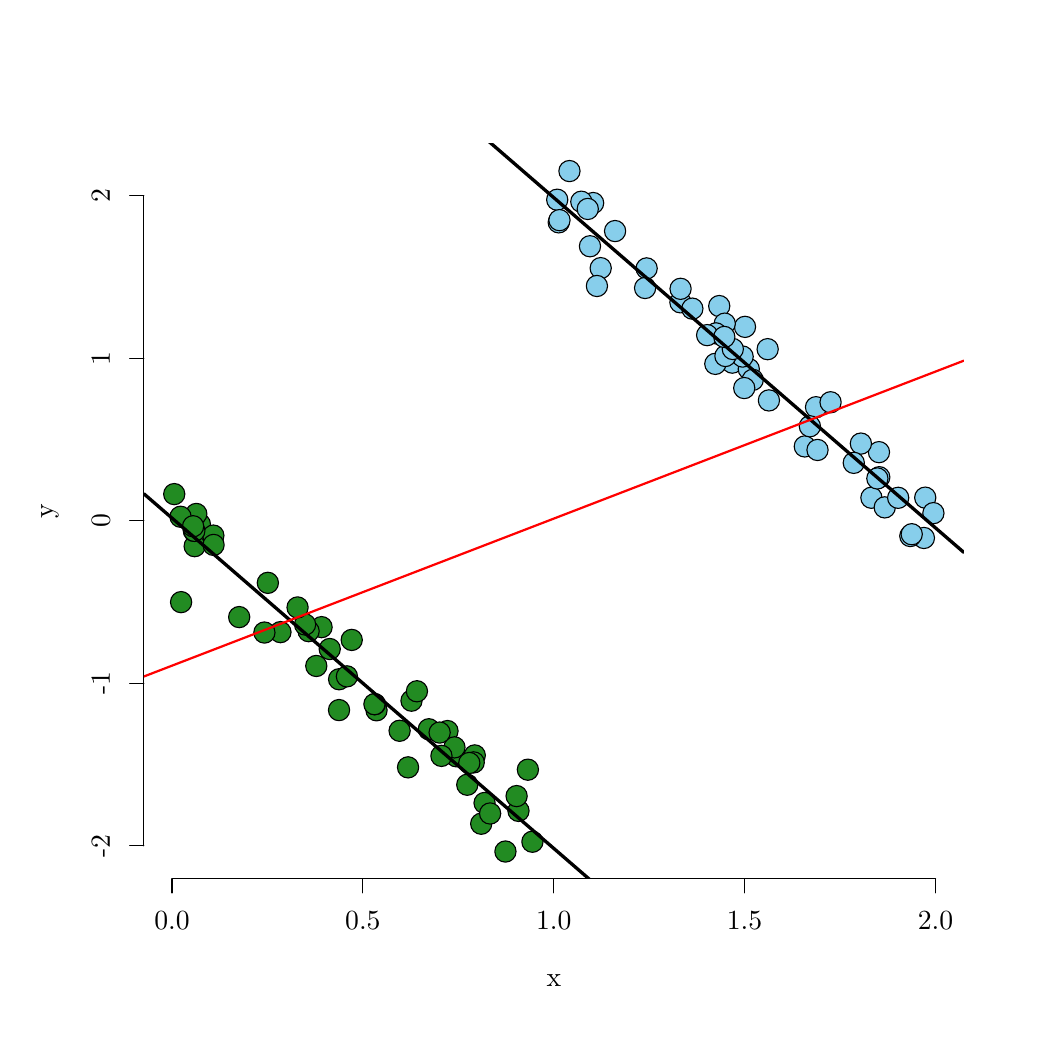
\begin{tikzpicture}[scale = 0.025]
% Created by tikzDevice version 0.12 on 2019-05-26 19:53:33
% !TEX encoding = UTF-8 Unicode
\definecolor{fillColor}{RGB}{255,255,255}
\path[use as bounding box,fill=fillColor,fill opacity=0.00] (0,0) rectangle (505.89,505.89);
\begin{scope}
\path[clip] (  0.00,  0.00) rectangle (505.89,505.89);
\definecolor{drawColor}{RGB}{0,0,0}

\path[draw=drawColor,line width= 0.4pt,line join=round,line cap=round] ( 73.36, 73.44) -- (461.26, 73.44);

\path[draw=drawColor,line width= 0.4pt,line join=round,line cap=round] ( 73.36, 73.44) -- ( 73.36, 66.24);

\path[draw=drawColor,line width= 0.4pt,line join=round,line cap=round] (170.34, 73.44) -- (170.34, 66.24);

\path[draw=drawColor,line width= 0.4pt,line join=round,line cap=round] (267.31, 73.44) -- (267.31, 66.24);

\path[draw=drawColor,line width= 0.4pt,line join=round,line cap=round] (364.28, 73.44) -- (364.28, 66.24);

\path[draw=drawColor,line width= 0.4pt,line join=round,line cap=round] (461.26, 73.44) -- (461.26, 66.24);

\node[text=drawColor,anchor=base,inner sep=0pt, outer sep=0pt, scale=  1.00] at ( 73.36, 47.52) {0.0};

\node[text=drawColor,anchor=base,inner sep=0pt, outer sep=0pt, scale=  1.00] at (170.34, 47.52) {0.5};

\node[text=drawColor,anchor=base,inner sep=0pt, outer sep=0pt, scale=  1.00] at (267.31, 47.52) {1.0};

\node[text=drawColor,anchor=base,inner sep=0pt, outer sep=0pt, scale=  1.00] at (364.28, 47.52) {1.5};

\node[text=drawColor,anchor=base,inner sep=0pt, outer sep=0pt, scale=  1.00] at (461.26, 47.52) {2.0};

\path[draw=drawColor,line width= 0.4pt,line join=round,line cap=round] ( 59.04, 90.11) -- ( 59.04,420.48);

\path[draw=drawColor,line width= 0.4pt,line join=round,line cap=round] ( 59.04, 90.11) -- ( 51.84, 90.11);

\path[draw=drawColor,line width= 0.4pt,line join=round,line cap=round] ( 59.04,172.70) -- ( 51.84,172.70);

\path[draw=drawColor,line width= 0.4pt,line join=round,line cap=round] ( 59.04,255.30) -- ( 51.84,255.30);

\path[draw=drawColor,line width= 0.4pt,line join=round,line cap=round] ( 59.04,337.89) -- ( 51.84,337.89);

\path[draw=drawColor,line width= 0.4pt,line join=round,line cap=round] ( 59.04,420.48) -- ( 51.84,420.48);

\node[text=drawColor,rotate= 90.00,anchor=base,inner sep=0pt, outer sep=0pt, scale=  1.00] at ( 41.76, 90.11) {-2};

\node[text=drawColor,rotate= 90.00,anchor=base,inner sep=0pt, outer sep=0pt, scale=  1.00] at ( 41.76,172.70) {-1};

\node[text=drawColor,rotate= 90.00,anchor=base,inner sep=0pt, outer sep=0pt, scale=  1.00] at ( 41.76,255.30) {0};

\node[text=drawColor,rotate= 90.00,anchor=base,inner sep=0pt, outer sep=0pt, scale=  1.00] at ( 41.76,337.89) {1};

\node[text=drawColor,rotate= 90.00,anchor=base,inner sep=0pt, outer sep=0pt, scale=  1.00] at ( 41.76,420.48) {2};
\end{scope}
\begin{scope}
\path[clip] (  0.00,  0.00) rectangle (505.89,505.89);
\definecolor{drawColor}{RGB}{0,0,0}

\node[text=drawColor,anchor=base,inner sep=0pt, outer sep=0pt, scale=  1.00] at (267.35, 18.72) {x};

\node[text=drawColor,rotate= 90.00,anchor=base,inner sep=0pt, outer sep=0pt, scale=  1.00] at ( 12.96,260.14) {y};
\end{scope}
\begin{scope}
\path[clip] ( 59.04, 73.44) rectangle (475.65,446.85);
\definecolor{drawColor}{RGB}{0,0,0}
\definecolor{fillColor}{RGB}{34,139,34}

\path[draw=drawColor,line width= 0.4pt,line join=round,line cap=round,fill=fillColor] ( 84.85,242.43) circle (  5.40);

\path[draw=drawColor,line width= 0.4pt,line join=round,line cap=round,fill=fillColor] (203.84,149.40) circle (  5.40);

\path[draw=drawColor,line width= 0.4pt,line join=round,line cap=round,fill=fillColor] (195.03,163.91) circle (  5.40);

\path[draw=drawColor,line width= 0.4pt,line join=round,line cap=round,fill=fillColor] ( 87.49,253.61) circle (  5.40);

\path[draw=drawColor,line width= 0.4pt,line join=round,line cap=round,fill=fillColor] (158.25,174.81) circle (  5.40);

\path[draw=drawColor,line width= 0.4pt,line join=round,line cap=round,fill=fillColor] (197.79,168.70) circle (  5.40);

\path[draw=drawColor,line width= 0.4pt,line join=round,line cap=round,fill=fillColor] (230.45,101.39) circle (  5.40);

\path[draw=drawColor,line width= 0.4pt,line join=round,line cap=round,fill=fillColor] (149.34,201.29) circle (  5.40);

\path[draw=drawColor,line width= 0.4pt,line join=round,line cap=round,fill=fillColor] (223.37,121.20) circle (  5.40);

\path[draw=drawColor,line width= 0.4pt,line join=round,line cap=round,fill=fillColor] (242.76, 87.27) circle (  5.40);

\path[draw=drawColor,line width= 0.4pt,line join=round,line cap=round,fill=fillColor] (193.28,130.04) circle (  5.40);

\path[draw=drawColor,line width= 0.4pt,line join=round,line cap=round,fill=fillColor] (142.74,199.24) circle (  5.40);

\path[draw=drawColor,line width= 0.4pt,line join=round,line cap=round,fill=fillColor] (254.17,128.85) circle (  5.40);

\path[draw=drawColor,line width= 0.4pt,line join=round,line cap=round,fill=fillColor] (217.80,135.66) circle (  5.40);

\path[draw=drawColor,line width= 0.4pt,line join=round,line cap=round,fill=fillColor] ( 85.69,258.80) circle (  5.40);

\path[draw=drawColor,line width= 0.4pt,line join=round,line cap=round,fill=fillColor] ( 94.35,247.81) circle (  5.40);

\path[draw=drawColor,line width= 0.4pt,line join=round,line cap=round,fill=fillColor] (232.16,111.94) circle (  5.40);

\path[draw=drawColor,line width= 0.4pt,line join=round,line cap=round,fill=fillColor] (227.18,136.11) circle (  5.40);

\path[draw=drawColor,line width= 0.4pt,line join=round,line cap=round,fill=fillColor] ( 84.44,250.23) circle (  5.40);

\path[draw=drawColor,line width= 0.4pt,line join=round,line cap=round,fill=fillColor] (249.39,107.93) circle (  5.40);

\path[draw=drawColor,line width= 0.4pt,line join=round,line cap=round,fill=fillColor] (213.32,148.49) circle (  5.40);

\path[draw=drawColor,line width= 0.4pt,line join=round,line cap=round,fill=fillColor] (248.44,115.44) circle (  5.40);

\path[draw=drawColor,line width= 0.4pt,line join=round,line cap=round,fill=fillColor] (177.26,159.04) circle (  5.40);

\path[draw=drawColor,line width= 0.4pt,line join=round,line cap=round,fill=fillColor] (140.96,202.62) circle (  5.40);

\path[draw=drawColor,line width= 0.4pt,line join=round,line cap=round,fill=fillColor] (234.98,106.60) circle (  5.40);

\path[draw=drawColor,line width= 0.4pt,line join=round,line cap=round,fill=fillColor] (226.65,132.56) circle (  5.40);

\path[draw=drawColor,line width= 0.4pt,line join=round,line cap=round,fill=fillColor] (176.43,162.15) circle (  5.40);

\path[draw=drawColor,line width= 0.4pt,line join=round,line cap=round,fill=fillColor] (224.39,132.26) circle (  5.40);

\path[draw=drawColor,line width= 0.4pt,line join=round,line cap=round,fill=fillColor] ( 84.68,250.21) circle (  5.40);

\path[draw=drawColor,line width= 0.4pt,line join=round,line cap=round,fill=fillColor] (162.21,176.27) circle (  5.40);

\path[draw=drawColor,line width= 0.4pt,line join=round,line cap=round,fill=fillColor] ( 77.69,257.37) circle (  5.40);

\path[draw=drawColor,line width= 0.4pt,line join=round,line cap=round,fill=fillColor] (216.86,140.19) circle (  5.40);

\path[draw=drawColor,line width= 0.4pt,line join=round,line cap=round,fill=fillColor] (210.24,135.86) circle (  5.40);

\path[draw=drawColor,line width= 0.4pt,line join=round,line cap=round,fill=fillColor] ( 74.47,268.88) circle (  5.40);

\path[draw=drawColor,line width= 0.4pt,line join=round,line cap=round,fill=fillColor] (164.66,194.79) circle (  5.40);

\path[draw=drawColor,line width= 0.4pt,line join=round,line cap=round,fill=fillColor] (188.99,148.62) circle (  5.40);

\path[draw=drawColor,line width= 0.4pt,line join=round,line cap=round,fill=fillColor] (128.44,198.75) circle (  5.40);

\path[draw=drawColor,line width= 0.4pt,line join=round,line cap=round,fill=fillColor] ( 84.07,252.54) circle (  5.40);

\path[draw=drawColor,line width= 0.4pt,line join=round,line cap=round,fill=fillColor] (146.65,181.56) circle (  5.40);

\path[draw=drawColor,line width= 0.4pt,line join=round,line cap=round,fill=fillColor] (176.20,162.14) circle (  5.40);

\path[draw=drawColor,line width= 0.4pt,line join=round,line cap=round,fill=fillColor] (122.04,223.79) circle (  5.40);

\path[draw=drawColor,line width= 0.4pt,line join=round,line cap=round,fill=fillColor] (256.47, 92.24) circle (  5.40);

\path[draw=drawColor,line width= 0.4pt,line join=round,line cap=round,fill=fillColor] (158.21,159.14) circle (  5.40);

\path[draw=drawColor,line width= 0.4pt,line join=round,line cap=round,fill=fillColor] (209.33,147.72) circle (  5.40);

\path[draw=drawColor,line width= 0.4pt,line join=round,line cap=round,fill=fillColor] (107.47,206.39) circle (  5.40);

\path[draw=drawColor,line width= 0.4pt,line join=round,line cap=round,fill=fillColor] (120.29,198.54) circle (  5.40);

\path[draw=drawColor,line width= 0.4pt,line join=round,line cap=round,fill=fillColor] ( 77.96,213.99) circle (  5.40);

\path[draw=drawColor,line width= 0.4pt,line join=round,line cap=round,fill=fillColor] (137.13,211.29) circle (  5.40);

\path[draw=drawColor,line width= 0.4pt,line join=round,line cap=round,fill=fillColor] (153.48,190.17) circle (  5.40);

\path[draw=drawColor,line width= 0.4pt,line join=round,line cap=round,fill=fillColor] ( 94.46,243.06) circle (  5.40);
\definecolor{fillColor}{RGB}{135,206,235}

\path[draw=drawColor,line width= 0.4pt,line join=round,line cap=round,fill=fillColor] (432.56,290.20) circle (  5.40);

\path[draw=drawColor,line width= 0.4pt,line join=round,line cap=round,fill=fillColor] (269.07,418.46) circle (  5.40);

\path[draw=drawColor,line width= 0.4pt,line join=round,line cap=round,fill=fillColor] (455.39,246.59) circle (  5.40);

\path[draw=drawColor,line width= 0.4pt,line join=round,line cap=round,fill=fillColor] (423.37,294.55) circle (  5.40);

\path[draw=drawColor,line width= 0.4pt,line join=round,line cap=round,fill=fillColor] (364.49,353.86) circle (  5.40);

\path[draw=drawColor,line width= 0.4pt,line join=round,line cap=round,fill=fillColor] (448.49,247.58) circle (  5.40);

\path[draw=drawColor,line width= 0.4pt,line join=round,line cap=round,fill=fillColor] (358.05,335.68) circle (  5.40);

\path[draw=drawColor,line width= 0.4pt,line join=round,line cap=round,fill=fillColor] (366.41,332.45) circle (  5.40);

\path[draw=drawColor,line width= 0.4pt,line join=round,line cap=round,fill=fillColor] (428.72,267.03) circle (  5.40);

\path[draw=drawColor,line width= 0.4pt,line join=round,line cap=round,fill=fillColor] (298.47,402.54) circle (  5.40);

\path[draw=drawColor,line width= 0.4pt,line join=round,line cap=round,fill=fillColor] (368.43,326.94) circle (  5.40);

\path[draw=drawColor,line width= 0.4pt,line join=round,line cap=round,fill=fillColor] (351.40,364.43) circle (  5.40);

\path[draw=drawColor,line width= 0.4pt,line join=round,line cap=round,fill=fillColor] (331.67,366.33) circle (  5.40);

\path[draw=drawColor,line width= 0.4pt,line join=round,line cap=round,fill=fillColor] (354.20,355.49) circle (  5.40);

\path[draw=drawColor,line width= 0.4pt,line join=round,line cap=round,fill=fillColor] (275.29,433.02) circle (  5.40);

\path[draw=drawColor,line width= 0.4pt,line join=round,line cap=round,fill=fillColor] (314.51,383.57) circle (  5.40);

\path[draw=drawColor,line width= 0.4pt,line join=round,line cap=round,fill=fillColor] (287.32,416.78) circle (  5.40);

\path[draw=drawColor,line width= 0.4pt,line join=round,line cap=round,fill=fillColor] (337.74,363.11) circle (  5.40);

\path[draw=drawColor,line width= 0.4pt,line join=round,line cap=round,fill=fillColor] (394.88,293.10) circle (  5.40);

\path[draw=drawColor,line width= 0.4pt,line join=round,line cap=round,fill=fillColor] (349.75,350.55) circle (  5.40);

\path[draw=drawColor,line width= 0.4pt,line join=round,line cap=round,fill=fillColor] (281.31,417.45) circle (  5.40);

\path[draw=drawColor,line width= 0.4pt,line join=round,line cap=round,fill=fillColor] (400.58,313.04) circle (  5.40);

\path[draw=drawColor,line width= 0.4pt,line join=round,line cap=round,fill=fillColor] (432.71,277.46) circle (  5.40);

\path[draw=drawColor,line width= 0.4pt,line join=round,line cap=round,fill=fillColor] (435.50,262.14) circle (  5.40);

\path[draw=drawColor,line width= 0.4pt,line join=round,line cap=round,fill=fillColor] (284.59,413.77) circle (  5.40);

\path[draw=drawColor,line width= 0.4pt,line join=round,line cap=round,fill=fillColor] (269.84,406.97) circle (  5.40);

\path[draw=drawColor,line width= 0.4pt,line join=round,line cap=round,fill=fillColor] (349.40,335.06) circle (  5.40);

\path[draw=drawColor,line width= 0.4pt,line join=round,line cap=round,fill=fillColor] (456.07,267.08) circle (  5.40);

\path[draw=drawColor,line width= 0.4pt,line join=round,line cap=round,fill=fillColor] (364.10,322.77) circle (  5.40);

\path[draw=drawColor,line width= 0.4pt,line join=round,line cap=round,fill=fillColor] (460.22,259.21) circle (  5.40);

\path[draw=drawColor,line width= 0.4pt,line join=round,line cap=round,fill=fillColor] (363.29,338.77) circle (  5.40);

\path[draw=drawColor,line width= 0.4pt,line join=round,line cap=round,fill=fillColor] (291.17,383.70) circle (  5.40);

\path[draw=drawColor,line width= 0.4pt,line join=round,line cap=round,fill=fillColor] (376.00,342.53) circle (  5.40);

\path[draw=drawColor,line width= 0.4pt,line join=round,line cap=round,fill=fillColor] (313.72,373.61) circle (  5.40);

\path[draw=drawColor,line width= 0.4pt,line join=round,line cap=round,fill=fillColor] (407.97,315.55) circle (  5.40);

\path[draw=drawColor,line width= 0.4pt,line join=round,line cap=round,fill=fillColor] (419.76,284.76) circle (  5.40);

\path[draw=drawColor,line width= 0.4pt,line join=round,line cap=round,fill=fillColor] (354.54,339.06) circle (  5.40);

\path[draw=drawColor,line width= 0.4pt,line join=round,line cap=round,fill=fillColor] (358.29,342.61) circle (  5.40);

\path[draw=drawColor,line width= 0.4pt,line join=round,line cap=round,fill=fillColor] (345.25,349.66) circle (  5.40);

\path[draw=drawColor,line width= 0.4pt,line join=round,line cap=round,fill=fillColor] (442.32,267.00) circle (  5.40);

\path[draw=drawColor,line width= 0.4pt,line join=round,line cap=round,fill=fillColor] (376.64,316.49) circle (  5.40);

\path[draw=drawColor,line width= 0.4pt,line join=round,line cap=round,fill=fillColor] (401.33,291.31) circle (  5.40);

\path[draw=drawColor,line width= 0.4pt,line join=round,line cap=round,fill=fillColor] (331.75,373.19) circle (  5.40);

\path[draw=drawColor,line width= 0.4pt,line join=round,line cap=round,fill=fillColor] (285.71,394.82) circle (  5.40);

\path[draw=drawColor,line width= 0.4pt,line join=round,line cap=round,fill=fillColor] (449.21,248.50) circle (  5.40);

\path[draw=drawColor,line width= 0.4pt,line join=round,line cap=round,fill=fillColor] (397.45,303.35) circle (  5.40);

\path[draw=drawColor,line width= 0.4pt,line join=round,line cap=round,fill=fillColor] (270.22,408.08) circle (  5.40);

\path[draw=drawColor,line width= 0.4pt,line join=round,line cap=round,fill=fillColor] (289.25,374.63) circle (  5.40);

\path[draw=drawColor,line width= 0.4pt,line join=round,line cap=round,fill=fillColor] (431.74,276.83) circle (  5.40);

\path[draw=drawColor,line width= 0.4pt,line join=round,line cap=round,fill=fillColor] (353.97,348.74) circle (  5.40);

\path[draw=drawColor,line width= 1.2pt,line join=round,line cap=round] ( 59.04,269.05) -- (370.02,  0.00);

\path[draw=drawColor,line width= 1.2pt,line join=round,line cap=round] (167.49,505.89) -- (475.65,239.28);
\definecolor{drawColor}{RGB}{255,0,0}

\path[draw=drawColor,line width= 0.8pt,line join=round,line cap=round] ( 59.04,176.20) -- (475.65,336.67);
\end{scope}

\end{tikzpicture}
\end{center}
\end{minipage}

\item А вот так не бывает!
\end{enumerate}
\end{sol}
\end{problem}




\begin{problem} %1.16
Вася оценил модель $y=\beta_1+\beta_2 d+\beta_3 x+\varepsilon$. Дамми-переменная $d$ обозначает пол, 1 для мужчин и 0 для женщин. Оказалось, что $\hb_2>0$. Означает ли это, что для мужчин $\bar{y}$ больше, чем $\bar{y}$ для женщин?


\begin{sol}
Нет. Коэффициенты можно интерпретировать только «при прочих равных», т.е. при равных $x$. Из-за разных $x$ может оказаться, что у мужчин $\bar{y}$ меньше, чем $\bar{y}$ для женщин.
\end{sol}
\end{problem}




\begin{problem} %1.17
Какие из указанные моделей можно представить в линейном виде?
\begin{enumerate}
\item $y_i=\beta_1+\frac{\beta_2}{x_i}+\e_i$;
\item $y_i=\exp(\beta_1+\beta_2 x_i+\e_i)$;
\item $y_i=1+\frac{1}{\exp(\beta_1+\beta_2 x_i+\e_i)}$;
\item $y_i=\frac{1}{1+\exp(\beta_1+\beta_2 x_i+\e_i)}$;
\item $y_i=x_i^{\beta_2}e^{\beta_1+\e_i}$;
\item $y_i=\beta_1\exp(\beta_2 x_i + \e_i)$.
\end{enumerate}


\begin{sol}
Модель можно представить в линейном виде, когда неизвестные параметры входят в нее линейно.
\begin{enumerate}
\item Обозначим $z_i = 1/x_i$, и готово.
\item Возьмем логарифм от обеих частей\ldots
\item Вычтем единицу из обеих частей и снова логарифм\ldots
\item Перевернем обе части уравнения, вычтем единицу и прологарифмируем\ldots
\item Вместо $x_i$ возьмем $e^{x_i}$ и прологарифмируем\ldots
\item Вместо $\beta_1$ возьмем $e^{\beta_1}$ и прологарифмируем\ldots
\end{enumerate}
\end{sol}
\end{problem}




\begin{problem} %1.18
У эконометриста Вовочки есть переменная $f_i$, которая равна 1, если $i$-ый человек в выборке — женщина, и 0, если мужчина. Есть переменная $m_i$, которая равна 1, если $i$-ый человек в выборке — мужчина, и 0, если женщина. Какие $\hy$ получатся, если Вовочка попытается построить регрессии:
\begin{enumerate}
\item $y$ на константу и $f$;
\item $y$ на константу и $m$;
\item $y$ на $f$ и $m$ без константы;
\item $y$ на константу, $f$ и $m$.
\end{enumerate}


\begin{sol}
Пусть \(\bar{y}_m\) — среднее значение \(y\) по выборке для мужчин, \(\bar{y}_f\) — среднее значение \(y\) по выборке для женщин. Тогда

\begin{enumerate}
\item \(\hy = \bar{y}_m + \left( \bar{y}_m -  \bar{y}_f \right) \cdot f \)

Оцениваемая модель:
\[
y_i = \beta_1 + \beta_2 f_i + \e_i 
\]

Стандартная процедура МНК:
\[RSS = \sum \e_i^2 = \sum \left(y_i - \beta_1 - \beta_2 \cdot f_i \right)^2 \rightarrow \min \limits_{\beta_1, \beta_2}\]
\[\frac{\partial RSS}{\partial \beta_1} = 2 \sum \left(y_i - \beta_1 - \beta_2\right)(-1) \]
\[\frac{\partial RSS}{\partial \beta_2} = 2 \sum \left(y_i - \beta_1 - \beta_2 \right)(-f_i) \]

Условия первого порядка:
\[\sum \left(y_i - \hb_1 - \hb_2 \cdot f_i\right) = 0\]
\[\sum \left(\left(y_i - \hb_1 - \hb_2 \cdot f_i\right)\cdot f_i\right)= 0\]

Осталось немного поработать с оператором суммирования. Обозначим за \(k\) — число женщин в нашей выборке объемом \(n\), мужчин тогда будет \(n - k\). Тогда
\[\sum \left(y_i - \hb_1 - \hb_2 \cdot f_i\right) = k \bar{y}_f + (n - k) \bar{y}_m - n \hb_1 - k \hb_2 = 0\]
\[\sum \left(\left(y_i - \hb_1 - \hb_2 \cdot f_i\right)\cdot f_i\right) = k \bar{y}_f - k \hb_1 - k \hb_2 =0\]

Отсюда легко ищутся оценки коэффициентов:
\[\hb_1 = \bar{y}_m, \ \hb_2 = \bar{y}_f - \bar{y}_m  \]

Следовательно:
\[\hy = \bar{y}_m + \left( \bar{y}_f -  \bar{y}_m \right) \cdot f \]

\item \(\hy = \bar{y}_f + \left( \bar{y}_m -  \bar{y}_f \right) \cdot m \)

\item \(\hy = \bar{y}_m \cdot m + \bar{y}_f \cdot f \)

\item Условия первого порядка линейного зависимы — мультиколлинеарность. МНК-оценки здесь не единственны.
\end{enumerate}
\end{sol}
\end{problem}




\begin{problem} %1.19
У эконометриста Вовочки есть три переменных: $r_i$ — доход $i$-го человека в выборке, $m_i$ — пол (1 — мальчик, 0 — девочка) и $f_i$ — пол (1 — девочка, 0 — мальчик). Вовочка оценил две модели
\begin{enumerate}
\item[] Модель A: $m_i=\beta_1+\beta_2 r_i+\ve_i$;
\item[] Модель B: $f_i=\gamma_1+\gamma_2 r_i+u_i$.
\end{enumerate}
\begin{enumerate}
\item Как связаны между собой оценки $\hb_1$ и $\hat{\gamma}_1$?
\item Как связаны между собой оценки $\hb_2$ и $\hat{\gamma}_2$?
\end{enumerate}


\begin{sol}
Если сложить попарно $m_i$ и $f_i$, то в сумме всегда выйдет единица. А оценки, полученные при помощи метода наименьших квадратов линейны по объясняемой переменной, то есть оценки коэффициентов модели $m_i+f_i \sim \dots$ это суммы соответствующих оценок из двух разных моделей. Но они должны получиться равными 1 и 0 соответствнно (так как зависимая переменная — вектор из единиц). Поэтому $\hb_1 + \hat{\gamma}_1 = 1$, $\hb_2 + \hat{\gamma}_2 = 0$.
\end{sol}
\end{problem}




\begin{problem} %1.20
Эконометрист Вовочка оценил линейную регрессионную модель, где $y$ измерялся в тугриках. Затем он оценил ту же модель, но измерял $y$ в мунгу (1 тугрик = 100 мунгу). Как изменятся оценки коэффициентов?


\begin{sol}
Все оценки коэффициентов увеличатся в 100 раз.
\end{sol}
\end{problem}



\begin{problem} %1.21
Возможно ли, что при оценке парной регрессии $y=\beta_1+\beta_2 x+\e$ оказывается, что $\hb_2>0$, а при оценке регрессии без константы, $y=\gamma x+\e$, оказывается, что $\hat{\gamma}<0$?


\begin{sol}
Да, возможно:

\begin{minted}[mathescape,
               linenos,
               numbersep=5pt,
               frame=lines,
               framesep=2mm]{r}
x <- c(rnorm(n, mean = 4, sd = 2))
y <- x - 7 + runif(n, min = -1, max = 1)

plot(x,y, pch = 21, bg = "ForestGreen",
     col = "black", xlim = c(0,10), ylim = c(-5,3))
abline(coef(lm(y ~ x))[1], coef(lm(y ~ x))[2], lwd = 2)
abline(0, coef(lm(y ~ 0 + x))[1] , lwd = 2)
labels <- c("With intercept", "Without intercept")
text(c(7.5, 1.5), c(2, 0.4), labels)
coef(lm(y ~ x))
coef(lm(y ~ 0 + x))
\end{minted}

\begin{minipage}{0.6\textwidth}
\begin{center}
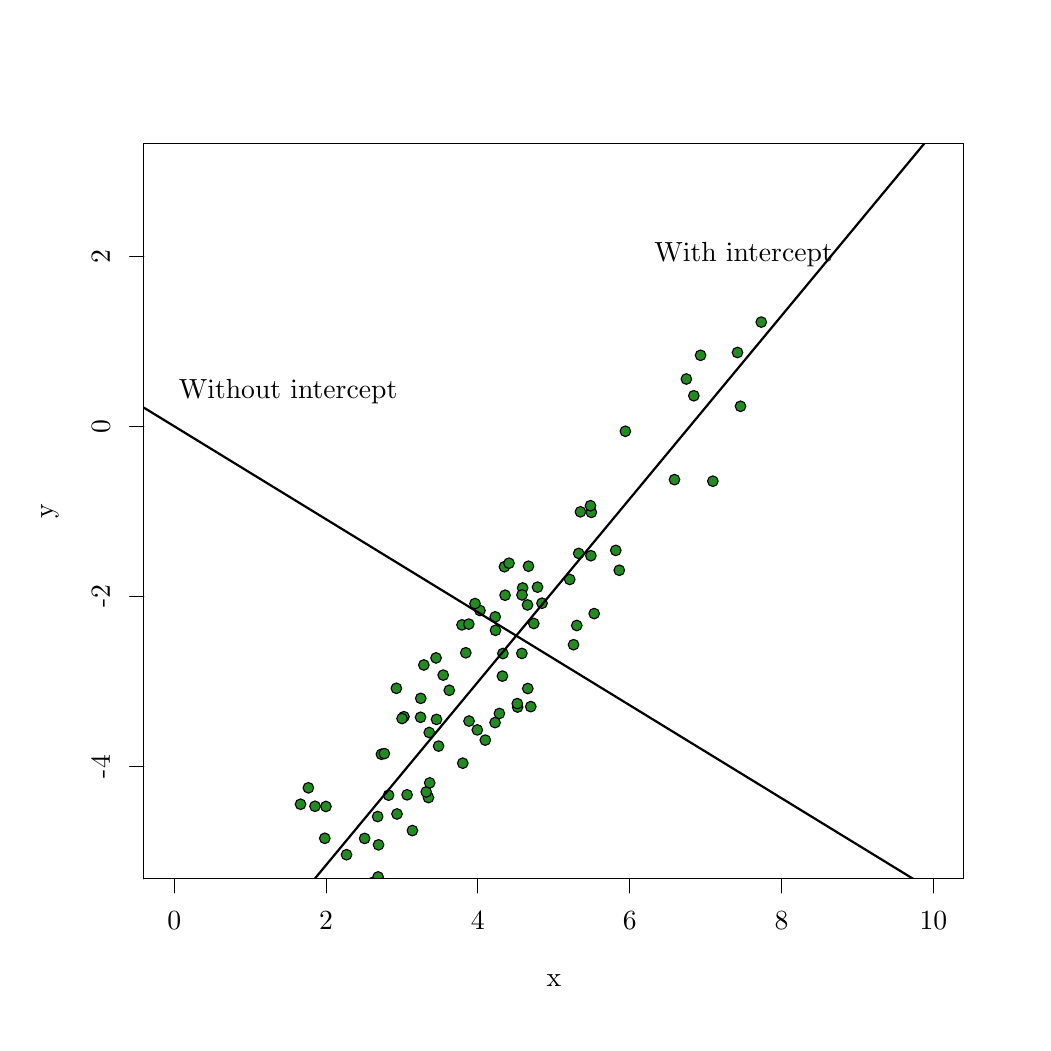
\begin{tikzpicture}[scale = 0.025]
% Created by tikzDevice version 0.12 on 2019-05-26 19:55:30
% !TEX encoding = UTF-8 Unicode
\definecolor{fillColor}{RGB}{255,255,255}
\path[use as bounding box,fill=fillColor,fill opacity=0.00] (0,0) rectangle (505.89,505.89);
\begin{scope}
\path[clip] ( 59.04, 73.44) rectangle (475.65,446.85);
\definecolor{drawColor}{RGB}{0,0,0}
\definecolor{fillColor}{RGB}{34,139,34}

\path[draw=drawColor,line width= 0.4pt,line join=round,line cap=round,fill=fillColor] (251.51,221.18) circle (  2.70);

\path[draw=drawColor,line width= 0.4pt,line join=round,line cap=round,fill=fillColor] (259.07,221.60) circle (  2.70);

\path[draw=drawColor,line width= 0.4pt,line join=round,line cap=round,fill=fillColor] (151.55,110.17) circle (  2.70);

\path[draw=drawColor,line width= 0.4pt,line join=round,line cap=round,fill=fillColor] (203.64,114.68) circle (  2.70);

\path[draw=drawColor,line width= 0.4pt,line join=round,line cap=round,fill=fillColor] (150.98, 93.99) circle (  2.70);

\path[draw=drawColor,line width= 0.4pt,line join=round,line cap=round,fill=fillColor] (179.75,136.70) circle (  2.70);

\path[draw=drawColor,line width= 0.4pt,line join=round,line cap=round,fill=fillColor] (135.43, 62.22) circle (  2.70);

\path[draw=drawColor,line width= 0.4pt,line join=round,line cap=round,fill=fillColor] (142.63,119.64) circle (  2.70);

\path[draw=drawColor,line width= 0.4pt,line join=round,line cap=round,fill=fillColor] (277.37,192.37) circle (  2.70);

\path[draw=drawColor,line width= 0.4pt,line join=round,line cap=round,fill=fillColor] (207.74,154.40) circle (  2.70);

\path[draw=drawColor,line width= 0.4pt,line join=round,line cap=round,fill=fillColor] (208.80,140.85) circle (  2.70);

\path[draw=drawColor,line width= 0.4pt,line join=round,line cap=round,fill=fillColor] (362.21,313.50) circle (  2.70);

\path[draw=drawColor,line width= 0.4pt,line join=round,line cap=round,fill=fillColor] (224.27,153.56) circle (  2.70);

\path[draw=drawColor,line width= 0.4pt,line join=round,line cap=round,fill=fillColor] (187.34,170.20) circle (  2.70);

\path[draw=drawColor,line width= 0.4pt,line join=round,line cap=round,fill=fillColor] (286.42,259.60) circle (  2.70);

\path[draw=drawColor,line width= 0.4pt,line join=round,line cap=round,fill=fillColor] (191.18,155.77) circle (  2.70);

\path[draw=drawColor,line width= 0.4pt,line join=round,line cap=round,fill=fillColor] (334.69,327.36) circle (  2.70);

\path[draw=drawColor,line width= 0.4pt,line join=round,line cap=round,fill=fillColor] (199.63,155.47) circle (  2.70);

\path[draw=drawColor,line width= 0.4pt,line join=round,line cap=round,fill=fillColor] (181.23,137.03) circle (  2.70);

\path[draw=drawColor,line width= 0.4pt,line join=round,line cap=round,fill=fillColor] (138.65,111.29) circle (  2.70);

\path[draw=drawColor,line width= 0.4pt,line join=round,line cap=round,fill=fillColor] (254.12,170.10) circle (  2.70);

\path[draw=drawColor,line width= 0.4pt,line join=round,line cap=round,fill=fillColor] (341.91,339.41) circle (  2.70);

\path[draw=drawColor,line width= 0.4pt,line join=round,line cap=round,fill=fillColor] (201.30,182.06) circle (  2.70);

\path[draw=drawColor,line width= 0.4pt,line join=round,line cap=round,fill=fillColor] (248.94,160.68) circle (  2.70);

\path[draw=drawColor,line width= 0.4pt,line join=round,line cap=round,fill=fillColor] (254.49,232.24) circle (  2.70);

\path[draw=drawColor,line width= 0.4pt,line join=round,line cap=round,fill=fillColor] (338.49,318.86) circle (  2.70);

\path[draw=drawColor,line width= 0.4pt,line join=round,line cap=round,fill=fillColor] (279.99,238.74) circle (  2.70);

\path[draw=drawColor,line width= 0.4pt,line join=round,line cap=round,fill=fillColor] (145.94, 64.05) circle (  2.70);

\path[draw=drawColor,line width= 0.4pt,line join=round,line cap=round,fill=fillColor] (175.00, 71.43) circle (  2.70);

\path[draw=drawColor,line width= 0.4pt,line join=round,line cap=round,fill=fillColor] (171.21, 93.93) circle (  2.70);

\path[draw=drawColor,line width= 0.4pt,line join=round,line cap=round,fill=fillColor] (239.69,157.41) circle (  2.70);

\path[draw=drawColor,line width= 0.4pt,line join=round,line cap=round,fill=fillColor] (228.47,149.06) circle (  2.70);

\path[draw=drawColor,line width= 0.4pt,line join=round,line cap=round,fill=fillColor] (257.16,203.15) circle (  2.70);

\path[draw=drawColor,line width= 0.4pt,line join=round,line cap=round,fill=fillColor] (178.06, 74.36) circle (  2.70);

\path[draw=drawColor,line width= 0.4pt,line join=round,line cap=round,fill=fillColor] (199.73,165.10) circle (  2.70);

\path[draw=drawColor,line width= 0.4pt,line join=round,line cap=round,fill=fillColor] (285.97,262.98) circle (  2.70);

\path[draw=drawColor,line width= 0.4pt,line join=round,line cap=round,fill=fillColor] (221.09,132.17) circle (  2.70);

\path[draw=drawColor,line width= 0.4pt,line join=round,line cap=round,fill=fillColor] (178.29, 90.67) circle (  2.70);

\path[draw=drawColor,line width= 0.4pt,line join=round,line cap=round,fill=fillColor] (303.70,300.81) circle (  2.70);

\path[draw=drawColor,line width= 0.4pt,line join=round,line cap=round,fill=fillColor] (229.81,209.73) circle (  2.70);

\path[draw=drawColor,line width= 0.4pt,line join=round,line cap=round,fill=fillColor] (158.06, 51.73) circle (  2.70);

\path[draw=drawColor,line width= 0.4pt,line join=round,line cap=round,fill=fillColor] (360.67,340.83) circle (  2.70);

\path[draw=drawColor,line width= 0.4pt,line join=round,line cap=round,fill=fillColor] (138.65, 64.68) circle (  2.70);

\path[draw=drawColor,line width= 0.4pt,line join=round,line cap=round,fill=fillColor] (279.00,202.12) circle (  2.70);

\path[draw=drawColor,line width= 0.4pt,line join=round,line cap=round,fill=fillColor] (187.66,106.35) circle (  2.70);

\path[draw=drawColor,line width= 0.4pt,line join=round,line cap=round,fill=fillColor] (207.51,185.64) circle (  2.70);

\path[draw=drawColor,line width= 0.4pt,line join=round,line cap=round,fill=fillColor] (251.11,187.93) circle (  2.70);

\path[draw=drawColor,line width= 0.4pt,line join=round,line cap=round,fill=fillColor] (192.78,116.08) circle (  2.70);

\path[draw=drawColor,line width= 0.4pt,line join=round,line cap=round,fill=fillColor] (104.71, 58.14) circle (  2.70);

\path[draw=drawColor,line width= 0.4pt,line join=round,line cap=round,fill=fillColor] (202.49,117.55) circle (  2.70);

\path[draw=drawColor,line width= 0.4pt,line join=round,line cap=round,fill=fillColor] (242.25,231.97) circle (  2.70);

\path[draw=drawColor,line width= 0.4pt,line join=round,line cap=round,fill=fillColor] (251.18,217.65) circle (  2.70);

\path[draw=drawColor,line width= 0.4pt,line join=round,line cap=round,fill=fillColor] (261.35,213.44) circle (  2.70);

\path[draw=drawColor,line width= 0.4pt,line join=round,line cap=round,fill=fillColor] (328.66,276.24) circle (  2.70);

\path[draw=drawColor,line width= 0.4pt,line join=round,line cap=round,fill=fillColor] (241.48,187.88) circle (  2.70);

\path[draw=drawColor,line width= 0.4pt,line join=round,line cap=round,fill=fillColor] (244.58,233.77) circle (  2.70);

\path[draw=drawColor,line width= 0.4pt,line join=round,line cap=round,fill=fillColor] (275.42,225.52) circle (  2.70);

\path[draw=drawColor,line width= 0.4pt,line join=round,line cap=round,fill=fillColor] (227.29,213.26) circle (  2.70);

\path[draw=drawColor,line width= 0.4pt,line join=round,line cap=round,fill=fillColor] (222.62,188.25) circle (  2.70);

\path[draw=drawColor,line width= 0.4pt,line join=round,line cap=round,fill=fillColor] (237.72,199.68) circle (  2.70);

\path[draw=drawColor,line width= 0.4pt,line join=round,line cap=round,fill=fillColor] (286.18,237.58) circle (  2.70);

\path[draw=drawColor,line width= 0.4pt,line join=round,line cap=round,fill=fillColor] (195.50, 97.92) circle (  2.70);

\path[draw=drawColor,line width= 0.4pt,line join=round,line cap=round,fill=fillColor] (190.23,154.83) circle (  2.70);

\path[draw=drawColor,line width= 0.4pt,line join=round,line cap=round,fill=fillColor] (162.02, 85.64) circle (  2.70);

\path[draw=drawColor,line width= 0.4pt,line join=round,line cap=round,fill=fillColor] (154.88, 49.62) circle (  2.70);

\path[draw=drawColor,line width= 0.4pt,line join=round,line cap=round,fill=fillColor] (253.98,212.57) circle (  2.70);

\path[draw=drawColor,line width= 0.4pt,line join=round,line cap=round,fill=fillColor] (348.15,275.44) circle (  2.70);

\path[draw=drawColor,line width= 0.4pt,line join=round,line cap=round,fill=fillColor] (154.02, 62.29) circle (  2.70);

\path[draw=drawColor,line width= 0.4pt,line join=round,line cap=round,fill=fillColor] (214.23,169.21) circle (  2.70);

\path[draw=drawColor,line width= 0.4pt,line join=round,line cap=round,fill=fillColor] (149.31, 56.04) circle (  2.70);

\path[draw=drawColor,line width= 0.4pt,line join=round,line cap=round,fill=fillColor] (298.83,240.28) circle (  2.70);

\path[draw=drawColor,line width= 0.4pt,line join=round,line cap=round,fill=fillColor] (204.28,122.15) circle (  2.70);

\path[draw=drawColor,line width= 0.4pt,line join=round,line cap=round,fill=fillColor] (242.58,217.50) circle (  2.70);

\path[draw=drawColor,line width= 0.4pt,line join=round,line cap=round,fill=fillColor] (255.62,160.89) circle (  2.70);

\path[draw=drawColor,line width= 0.4pt,line join=round,line cap=round,fill=fillColor] (147.43, 52.97) circle (  2.70);

\path[draw=drawColor,line width= 0.4pt,line join=round,line cap=round,fill=fillColor] (220.69,202.44) circle (  2.70);

\path[draw=drawColor,line width= 0.4pt,line join=round,line cap=round,fill=fillColor] (211.15,176.91) circle (  2.70);

\path[draw=drawColor,line width= 0.4pt,line join=round,line cap=round,fill=fillColor] (280.87,259.88) circle (  2.70);

\path[draw=drawColor,line width= 0.4pt,line join=round,line cap=round,fill=fillColor] (133.63, 45.66) circle (  2.70);

\path[draw=drawColor,line width= 0.4pt,line join=round,line cap=round,fill=fillColor] (136.19, 36.93) circle (  2.70);

\path[draw=drawColor,line width= 0.4pt,line join=round,line cap=round,fill=fillColor] (287.86,208.17) circle (  2.70);

\path[draw=drawColor,line width= 0.4pt,line join=round,line cap=round,fill=fillColor] (183.40,115.90) circle (  2.70);

\path[draw=drawColor,line width= 0.4pt,line join=round,line cap=round,fill=fillColor] (177.83,105.04) circle (  2.70);

\path[draw=drawColor,line width= 0.4pt,line join=round,line cap=round,fill=fillColor] (237.49,152.77) circle (  2.70);

\path[draw=drawColor,line width= 0.4pt,line join=round,line cap=round,fill=fillColor] (204.05,147.73) circle (  2.70);

\path[draw=drawColor,line width= 0.4pt,line join=round,line cap=round,fill=fillColor] (372.76,356.28) circle (  2.70);

\path[draw=drawColor,line width= 0.4pt,line join=round,line cap=round,fill=fillColor] (248.79,162.41) circle (  2.70);

\path[draw=drawColor,line width= 0.4pt,line join=round,line cap=round,fill=fillColor] (241.23,176.40) circle (  2.70);

\path[draw=drawColor,line width= 0.4pt,line join=round,line cap=round,fill=fillColor] (300.60,230.19) circle (  2.70);

\path[draw=drawColor,line width= 0.4pt,line join=round,line cap=round,fill=fillColor] (224.15,202.84) circle (  2.70);

\path[draw=drawColor,line width= 0.4pt,line join=round,line cap=round,fill=fillColor] (232.53,143.89) circle (  2.70);

\path[draw=drawColor,line width= 0.4pt,line join=round,line cap=round,fill=fillColor] (146.00,110.27) circle (  2.70);

\path[draw=drawColor,line width= 0.4pt,line join=round,line cap=round,fill=fillColor] ( 51.87,  5.36) circle (  2.70);

\path[draw=drawColor,line width= 0.4pt,line join=round,line cap=round,fill=fillColor] (135.63, 28.47) circle (  2.70);

\path[draw=drawColor,line width= 0.4pt,line join=round,line cap=round,fill=fillColor] (237.57,206.51) circle (  2.70);

\path[draw=drawColor,line width= 0.4pt,line join=round,line cap=round,fill=fillColor] (149.05, 64.93) circle (  2.70);
\end{scope}
\begin{scope}
\path[clip] (  0.00,  0.00) rectangle (505.89,505.89);
\definecolor{drawColor}{RGB}{0,0,0}

\path[draw=drawColor,line width= 0.4pt,line join=round,line cap=round] ( 74.47, 73.44) -- (460.22, 73.44);

\path[draw=drawColor,line width= 0.4pt,line join=round,line cap=round] ( 74.47, 73.44) -- ( 74.47, 66.24);

\path[draw=drawColor,line width= 0.4pt,line join=round,line cap=round] (151.62, 73.44) -- (151.62, 66.24);

\path[draw=drawColor,line width= 0.4pt,line join=round,line cap=round] (228.77, 73.44) -- (228.77, 66.24);

\path[draw=drawColor,line width= 0.4pt,line join=round,line cap=round] (305.92, 73.44) -- (305.92, 66.24);

\path[draw=drawColor,line width= 0.4pt,line join=round,line cap=round] (383.07, 73.44) -- (383.07, 66.24);

\path[draw=drawColor,line width= 0.4pt,line join=round,line cap=round] (460.22, 73.44) -- (460.22, 66.24);

\node[text=drawColor,anchor=base,inner sep=0pt, outer sep=0pt, scale=  1.00] at ( 74.47, 47.52) {0};

\node[text=drawColor,anchor=base,inner sep=0pt, outer sep=0pt, scale=  1.00] at (151.62, 47.52) {2};

\node[text=drawColor,anchor=base,inner sep=0pt, outer sep=0pt, scale=  1.00] at (228.77, 47.52) {4};

\node[text=drawColor,anchor=base,inner sep=0pt, outer sep=0pt, scale=  1.00] at (305.92, 47.52) {6};

\node[text=drawColor,anchor=base,inner sep=0pt, outer sep=0pt, scale=  1.00] at (383.07, 47.52) {8};

\node[text=drawColor,anchor=base,inner sep=0pt, outer sep=0pt, scale=  1.00] at (460.22, 47.52) {10};

\path[draw=drawColor,line width= 0.4pt,line join=round,line cap=round] ( 59.04,130.49) -- ( 59.04,389.80);

\path[draw=drawColor,line width= 0.4pt,line join=round,line cap=round] ( 59.04,130.49) -- ( 51.84,130.49);

\path[draw=drawColor,line width= 0.4pt,line join=round,line cap=round] ( 59.04,216.93) -- ( 51.84,216.93);

\path[draw=drawColor,line width= 0.4pt,line join=round,line cap=round] ( 59.04,303.36) -- ( 51.84,303.36);

\path[draw=drawColor,line width= 0.4pt,line join=round,line cap=round] ( 59.04,389.80) -- ( 51.84,389.80);

\node[text=drawColor,rotate= 90.00,anchor=base,inner sep=0pt, outer sep=0pt, scale=  1.00] at ( 41.76,130.49) {-4};

\node[text=drawColor,rotate= 90.00,anchor=base,inner sep=0pt, outer sep=0pt, scale=  1.00] at ( 41.76,216.93) {-2};

\node[text=drawColor,rotate= 90.00,anchor=base,inner sep=0pt, outer sep=0pt, scale=  1.00] at ( 41.76,303.36) {0};

\node[text=drawColor,rotate= 90.00,anchor=base,inner sep=0pt, outer sep=0pt, scale=  1.00] at ( 41.76,389.80) {2};

\path[draw=drawColor,line width= 0.4pt,line join=round,line cap=round] ( 59.04, 73.44) --
	(475.65, 73.44) --
	(475.65,446.85) --
	( 59.04,446.85) --
	( 59.04, 73.44);
\end{scope}
\begin{scope}
\path[clip] (  0.00,  0.00) rectangle (505.89,505.89);
\definecolor{drawColor}{RGB}{0,0,0}

\node[text=drawColor,anchor=base,inner sep=0pt, outer sep=0pt, scale=  1.00] at (267.35, 18.72) {x};

\node[text=drawColor,rotate= 90.00,anchor=base,inner sep=0pt, outer sep=0pt, scale=  1.00] at ( 12.96,260.14) {y};
\end{scope}
\begin{scope}
\path[clip] ( 59.04, 73.44) rectangle (475.65,446.85);
\definecolor{drawColor}{RGB}{0,0,0}

\path[draw=drawColor,line width= 0.8pt,line join=round,line cap=round] ( 84.98,  0.00) -- (475.65,471.20);

\path[draw=drawColor,line width= 0.8pt,line join=round,line cap=round] ( 59.04,312.81) -- (475.65, 57.64);

\node[text=drawColor,anchor=base,inner sep=0pt, outer sep=0pt, scale=  1.00] at (363.78,386.83) {With intercept};

\node[text=drawColor,anchor=base,inner sep=0pt, outer sep=0pt, scale=  1.00] at (132.33,317.68) {Without intercept};
\end{scope}

\end{tikzpicture}
\end{center}
\end{minipage}
\end{sol}
\end{problem}




\begin{problem} %1.22
Эконометрист Вовочка оценил регрессию $y$ только на константу. Какой коэффициент $R^2$ он получит?


\begin{sol}
Так как \(\hy = \hb = \bar{y} \), то \(R^2 = 0\).
\end{sol}
\end{problem}




\begin{problem} %1.23
Эконометрист Вовочка оценил методом наименьших квадратов модель 1, $y_i=\b_1+\b_2 x_i+\b_3 z_i+\e_i$, 
а затем модель 2, $y_i=\b_1+\b_2 x_i+\b_3 z_i+\b_4 w_i+\e_i$. 
Сравните полученные $ESS$, $RSS$, $TSS$ и $R^2$.


\begin{sol}
Вспомним формулу для  $TSS$:
\[
TSS = \sum\limits_{i=1}^n (y_i-\bar{y})^2
\]
Так как значения $y$ остались теми же, $TSS_1 = TSS_2$.

\[
RSS = \sum\limits_{i=1}^n (y_i-\hy_i)^2 \hspace{2cm} ESS = \sum\limits_{i=1}^n (\hy_i-\bar{y})^2
\]

Добавление еще одного регрессора не уменьшит точность оценки, то есть $RSS_2\leqslant RSS_1$, $ESS_2 \geqslant ESS_1$.

Соответственно, коэффициент $R^2 = ESS/TSS$ не уменьшится, то есть $R^2_2 \geqslant R^2_1$.

\end{sol}
\end{problem}





\begin{problem} %1.24
Создайте набор данных с тремя переменными $y$, $x$ и $z$ со следующими свойствами. При оценке модели $\hy=\hb_1+\hb_2 x$ получается $\hb_2>0$. При оценке модели $\hy=\hat{\gamma}_1+ \hat{\gamma}_2 x+\hat{\gamma}_3 z$ получается $\hat{\gamma}_2<0$. Объясните принцип, руководствуясь которым легко создать такой набор данных.


\begin{sol}
  Интересный результат, \cite{leamer1975result}: смена знака коэффициента перед \(x\) при удалении переменной \(z\) не может произойти, если абсолютное значение \(t\)-статистики коэффициента перед \(z\) в регрессии с регрессорами \(x\) и \(z\) меньше абсолютного значения \(t\)-статистики коэффициента перед \(x\).
Пример такого набора данных:
\begin{minted}[mathescape,
               linenos,
               numbersep=5pt,
               frame=lines,
               framesep=2mm]{r}
set.seed(777)
y <- 1:50
z <- y + rnorm(length(y), 0, 0.01)
x <- y + rnorm(length(y), 0, 1)
m_short <- lm(y ~ x)
m_long <- lm(y ~ x + z)
texreg(list(m_short, m_long))
\end{minted}

\begin{table}
\begin{center}
\begin{tabular}{l c c }
\hline
 & Model 1 & Model 2 \\
\hline
(Intercept) & $0.04$       & $-0.00$      \\
            & $(0.27)$     & $(0.00)$     \\
x           & $1.00^{***}$ & $-0.00$      \\
            & $(0.01)$     & $(0.00)$     \\
z           &              & $1.00^{***}$ \\
            &              & $(0.00)$     \\
\hline
R$^2$       & 1.00         & 1.00         \\
Adj. R$^2$  & 1.00         & 1.00         \\
Num. obs.   & 50           & 50           \\
RMSE        & 0.94         & 0.01         \\
\hline
\multicolumn{3}{l}{\scriptsize{$^{***}p<0.001$, $^{**}p<0.01$, $^*p<0.05$}}
\end{tabular}
\caption{Statistical models}
\label{table:coefficients}
\end{center}
\end{table}


\end{sol}
\end{problem}



\begin{problem} %1.25
У меня есть набор данных с выборочным средним $\bar{y}$ и выборочной дисперсией $s_y^2$. Как нужно преобразовать данные, чтобы выборочное среднее равнялось $7$, а выборочная дисперсия — $9$?


\begin{sol}
$y_i^*=7+3(y_i-\bar{y})/s_y$
% эта задача не использует понятия вероятностей, хотя близка. Пусть будет в невероятностной секции.
Нужно вспомнить свойства математического ожидания и дисперсии и провести следующие преобразования:
\[
\tilde{y}_i = \frac{y_i-\bar{y}}{s_y} \Rightarrow \E[\tilde{y}] = 0, \hspace{2mm} \Var(\tilde{y}) = 1
\]
\[
y^*_i = \tilde{y}_i\cdot3 + 7 \Rightarrow \E[y^*] = 7, \hspace{2mm} \Var(y^*) = 9
\]
\end{sol}
\end{problem}



\begin{problem} %1.26
Эконометресса Анжела оценила две парных регрессии $\hy_i = 2 - 3 x_i$  и $\hat x_i = 5 - \frac{1}{12}y_i$. Найдите $R^2$ в каждой регрессии и выборочную корреляцию между $x_i$ и $y_i$.
\begin{sol}

$R^2$ одинаков для этих моделей. Докажем это в общем виде.

$R^2$ для модели $\hy_i = \hb_1 +\hb_2 x_i$:

\begin{math}
R^2 = \frac{ESS}{TSS}= \frac{\sum\limits_{i=1}^n (\hat{y_i} - \bar{y})^2}{\sum\limits_{i=1}^n(y_i-\bar{y})^2}=\frac{\sum\limits_{i=1}^n(\hb_1 + \hb_2x_i - \bar{y})^2}{\sum\limits_{i=1}^n(y_i-\bar{y})^2}=\frac{\sum\limits_{i=1}^n(\bar{y} - \hb_2\bar{x} + \hb_2x_i - \bar{y})^2}{\sum\limits_{i=1}^n(y_i-\bar{y})^2}  = \frac{\hb_2^2 \sum\limits_{i=1}^n(x_i - \bar{x})^2}{\sum\limits_{i=1}^n(y_i-\bar{y})^2} = \\ = \frac{ \left( \sum\limits_{i=1}^n(x_i-\bar{x})(y_i - \bar{y}) \right)^2 \sum\limits_{i=1}^n(x_i - \bar{x})^2}{\left( \sum\limits_{i=1}^n(x_i - \bar{x})^2 \right)^2 \sum\limits_{i=1}^n(y_i-\bar{y})^2} = \frac{ \left( \sum\limits_{i=1}^n(x_i-\bar{x})(y_i - \bar{y}) \right)^2}{\sum\limits_{i=1}^n(x_i - \bar{x})^2 = \sum\limits_{i=1}^n(y_i-\bar{y})^2} = \frac{\sum\limits_{i=1}^n(x_i-\bar{x})(y_i - \bar{y})}{\sum\limits_{i=1}^n(x_i - \bar{x})^2} \frac{\sum\limits_{i=1}^n(x_i-\bar{x})(y_i - \bar{y})}{\sum\limits_{i=1}^n(y_i-\bar{y})^2} = \\ = \hb_2 \hat{\alpha}_2
\end{math}

Если проделать те же действия для модели $\hat x_i = \hat{\alpha}_1 +\hat{\alpha}_2 x_i$, мы получим тот же результат.

$R^2 = -3 \cdot \frac{-1}{12}=\frac{1}{4}$.

Также можно заметить, что $\hCorr^2 = R^2$. То есть, выборочная корреляция равна $-1/2$, так как коэффициенты отрицательные (между \(y\) и \(x\) отрицательная зависимость).
\end{sol}
\end{problem}

\begin{problem} %1.27
На работе Феофан построил парную регрессию по трём наблюдениям и посчитал прогнозы $\hy_i$. Придя домой он отчасти вспомнил результаты:

\begin{tabular}{rr}
\toprule
$y_i$ & $\hy_i$ \\
\midrule
$0$ & $1$ \\
$6$ & ? \\
$6$ & ? \\
\bottomrule
\end{tabular}

Поднапрягшись, Феофан вспомнил, что третий прогноз был больше второго. Помогите Феофану восстановить пропущенные значения.


\begin{sol}
На две неизвестных $a$ и $b$ нужно два уравнения. Эти два уравнения — ортогональность вектора остатков плоскости регрессоров. А именно:

\[
\begin{cases}
\sum_i (y_i - \hy_i) = 0 \\
\sum_i (y_i - \hy_i) \hy_i = 0 \\
\end{cases}
\]

В нашем случае

\[
\begin{cases}
-1 +(6-a) + (6-b) = 0 \\
-1 + (6 - a)a + (6-b)b = 0 \\
\end{cases}
\]

Решаем квадратное уравнение и получаем два решения: $a=4$ и $a=7$. Итого: $a=4$, $b=7$.
\end{sol}
\end{problem}


\begin{problem}
Вся выборка поделена на две части. Возможны ли такие ситуации:
\begin{enumerate}
\item Выборочная корреляция между $y$ и $x$ примерно равна нулю в каждой части, а по всей выборке примерно равна единице;
\item Выборочная корреляция между $y$ и $x$ примерно ранва единице в каждой части, а по всей выборке примерно равна нулю?
\end{enumerate}

\begin{sol}
Обе ситуации возможны.
\end{sol}
\end{problem}


\begin{problem}
Илон Маск оценил модель парной регрессии $y_i = \b_1 + \b_2 x_i + u_i$.
Часть данных и прогнозов окалазась потеряна. 

\begin{tabular}{ccc}
       \toprule
       $x_i$ & $y_i$ & $\hy_i$ \\
       \midrule
       $a$ & 6 & 1 \\
       1 & 7 & 0 \\
       1 & 4 & 3 \\
       2 & 5 & $b$ \\
       \bottomrule
\end{tabular}
       
Помогите бравому Илону Маску восстановить пропуски, найдите $a$ и $b$. 
\begin{sol}
Решаем систему двух уравнений:
\[
\begin{cases}
       \langle x, y - \hy \rangle = 0, \\
       \langle \ones, y - \hy \rangle = 0 
\end{cases}
\]

Из $\langle \ones, y - \hy \rangle = 0$ следует, что $b=18$. 
Затем из $\langle x, y - \hy \rangle = 0$ следует, что $a=18/5$.
\end{sol}
\end{problem}
       




\Closesolutionfile{solution_file}
